\documentclass[aps,pra,twocolumn,reprint,floatfix,amsmath,amssymb]{revtex4-2}

\usepackage{graphicx}
\usepackage{booktabs}
\usepackage{siunitx}
\usepackage[colorlinks=true,linkcolor=blue,citecolor=blue,urlcolor=blue,hypertexnames=false]{hyperref}
\usepackage{float}
\usepackage{xcolor}

\DeclareSIUnit\GHz{\giga\hertz}
\DeclareSIUnit\MHz{\mega\hertz}
\DeclareSIUnit\kHz{\kilo\hertz}
\DeclareSIUnit\ns{\nano\second}
\DeclareSIUnit\us{\micro\second}

\begin{document}

\title{Fast and Robust Active Cooling of a Storage Cavity in a\\Transmon-Storage-Readout cQED System}
\author{Execution Engineer}
\affiliation{Shyam Shankar Quantum Circuits Group}
\date{\today}

\begin{abstract}
We compare four active-cooling architectures for resetting a storage cavity to vacuum in a dispersively coupled transmon-storage-readout circuit-QED device: a pulsed sequential ladder, a continuous resonant bright-state protocol, a continuous detuned Raman-like protocol, and an auxiliary idealized autonomous benchmark.
Candidate operating points are selected by scanning over sideband coupling strength and detuning, and schemes are ranked by a composite robustness score that weights residual storage occupation, ground-state vacuum fidelity, and sensitivity to transmon decoherence and calibration offsets.
On the present device abstraction, the continuous Raman-like protocol achieves the highest robustness score ($0.982$) among the physical schemes, the pulsed ladder is the fastest practical protocol (e-fold time $\tau_e = \SI{11.0}{ns}$), and the resonant bright-state path comes close in raw e-fold time ($\tau_e = \SI{13.0}{ns}$) but carries significantly higher transmon excitation.
Readout-linewidth sweeps show that strengthening the readout dissipation from $1\times$ to $4\times$ reduces the Raman-like residual occupation by a factor of ${\sim}25$, confirming that the readout bath is the dominant lever for approaching the autonomous-cooling limit.
Convergence tests at time steps $\Delta t = 0.5$, $1.0$, and $\SI{2.0}{ns}$ and at two Hilbert-space truncations show that the e-fold-time ranking and truncation dependence are stable for $\Delta t \leq \SI{1.0}{ns}$, while the end-of-window residual occupations of the continuous protocols remain quantitatively time-step sensitive and are therefore quoted from the finer $\Delta t = \SI{0.5}{ns}$ baseline.
Coherence and calibration robustness sweeps ($T_1$ and $T_2$ scaling from $0.5\times$ to $2\times$; amplitude offsets $\pm 10\%$; detuning errors $\pm\SI{2}{MHz}$) provide sensitivity bands for each scheme's composite score, confirming that the Raman-like ranking advantage is maintained across the tested perturbation envelope.
\end{abstract}

\maketitle

%% ===================================================================
\section{Introduction}
\label{sec:intro}
%% ===================================================================

Active reset of bosonic modes is a central primitive in circuit-QED quantum information processing.
High-fidelity preparation of the cavity vacuum state is required at the start of every error-correction cycle~\cite{ofek2016extending}, between successive gate sequences in bosonic-code architectures~\cite{eickbusch2022fast,heeres2015snap}, and for multi-mode memory platforms where passive relaxation would exceed the duty cycle~\cite{huang2025fastsideband,Reagor2016}.

The simplest approach---waiting for the cavity to decay at its intrinsic rate $\kappa_s$---is impractical for high-$Q$ storage modes with photon lifetimes exceeding \SI{100}{\us}.
An alternative is to use the transmon as a nonlinear mediator to shuttle photons from the storage cavity into a lossy readout resonator, where they are rapidly dissipated.
This strategy was pioneered for qubit reset~\cite{reed2010fast,geerlings2013demonstrating,magnard2018reset} and extended to driven readout-resonator depletion~\cite{mcclure2016rapid}, but the design space for \emph{cavity} reset remains less systematically explored.

Several physical mechanisms are available.
\emph{Pulsed ladders} use number-resolved $\pi$-pulses to transfer population one Fock state at a time through the transmon into the readout~\cite{huang2025fastsideband}.
\emph{Continuous sideband} protocols apply a constant drive that mediates a two-photon process coupling storage and readout via the transmon; depending on whether the transmon is resonantly or virtually excited,  these range from a bright-state (large real transmon population) to a Raman-like (mostly virtual transmon population) regime.
The limiting case---an effective autonomous damping channel $\dot{\rho} \propto \mathcal{D}[a_s]\rho$---corresponds to perfect reservoir engineering~\cite{poyatos1996quantum,leghtas2015confining} and sets an upper bound, but is not natively available as a single device control.

This study asks which architecture gives the best speed-versus-robustness tradeoff when transmon decoherence ($T_1$, $T_2$), calibration offsets, and readout bath engineering are all included.
We systematically scan the operating-point space for each scheme, construct a composite robustness score from coherence and calibration sweeps, and present convergence and sensitivity analyses that quantify the confidence in the resulting ranking.

%% ===================================================================
\section{System and Methods}
\label{sec:methods}
%% ===================================================================

\subsection{Device Model}
\label{sec:device}

We model a three-mode circuit-QED device consisting of a storage cavity ($s$), a transmon qubit ($q$), and a readout resonator ($r$), following the standard dispersive Hamiltonian~\cite{blais2004cavity,blais2021circuit,koch2007transmon}:
\begin{align}
\label{eq:hamiltonian}
\hat{H}/\hbar &= \omega_s \hat{a}_s^\dagger \hat{a}_s + \omega_r \hat{a}_r^\dagger \hat{a}_r + \sum_j \omega_j |j\rangle\langle j| \nonumber \\
&\quad + \chi_{sr} \hat{a}_s^\dagger \hat{a}_s \hat{a}_r^\dagger \hat{a}_r + \chi_s \hat{a}_s^\dagger \hat{a}_s \hat{\sigma}_z + \chi_r \hat{a}_r^\dagger \hat{a}_r \hat{\sigma}_z \nonumber \\
&\quad + \hat{H}_{\mathrm{drive}}(t),
\end{align}
where $\hat{a}_{s,r}$ are annihilation operators for the storage and readout modes, $|j\rangle$ are transmon levels ($j \in \{g, e, f, h, \ldots\}$), and $\chi_s$, $\chi_r$ are the dispersive shifts.
The simulation is carried out in the \texttt{cqed\_sim} framework~\cite{cqedsim2026}, which handles the Lindblad master equation, sideband drive specifications, and rotating-frame transformations.

Table~\ref{tab:device} lists the device parameters used throughout this study.
These values are representative of a transmon-storage-readout device with a high-$Q$ storage cavity and a moderately lossy readout resonator~\cite{Reagor2016,krantz2019quantum}.

\begin{table}[t]
\caption{Device parameters used in all simulations.}
\label{tab:device}
\begin{tabular}{lcc}
\toprule
Parameter & Symbol & Value \\
\midrule
Storage frequency          & $\omega_s / 2\pi$       & \SI{5.241}{\GHz}   \\
Qubit frequency            & $\omega_q / 2\pi$       & \SI{6.150}{\GHz}   \\
Readout frequency          & $\omega_r / 2\pi$       & \SI{8.596}{\GHz}   \\
Qubit anharmonicity        & $\alpha_q / 2\pi$       & \SI{-255.67}{\MHz} \\
Storage dispersive shift   & $\chi_s / 2\pi$         & \SI{-2.840}{\MHz}  \\
Readout dispersive shift   & $\chi_r / 2\pi$         & \SI{-3.0}{\MHz}    \\
Readout linewidth          & $\kappa_r / 2\pi$       & \SI{4.156}{\MHz}   \\
Storage $T_1$              & $T_{1,s}$               & \SI{250}{\us}      \\
Storage $T_{2,\mathrm{R}}$ & $T_{2,s}$               & \SI{150}{\us}      \\
Transmon $T_1$             & $T_{1,q}$               & \SI{9.81}{\us}     \\
Transmon $T_{2,\mathrm{R}}$& $T_{2,q}$               & \SI{6.32}{\us}     \\
Transmon $T_{2,\mathrm{E}}$& $T_{2,q}^{(\mathrm{E})}$ & \SI{8.38}{\us}     \\
\bottomrule
\end{tabular}
\end{table}

\subsection{Compared Schemes}
\label{sec:schemes}

\begin{enumerate}
\item \textbf{Pulsed ladder.}  A sequence of number-resolved $\pi$-pulses transfers storage population through $|g,0_r,n_s\rangle \to |f,0_r,n_s{-}1\rangle$, followed by a readout-sideband swap $|f,0_r\rangle \to |g,1_r\rangle$ and readout ringdown $|1_r\rangle \xrightarrow{\kappa_r} |0_r\rangle$.
Each step is short, and the protocol scales linearly with the initial Fock number.

\item \textbf{Continuous resonant (bright-state).}  A constant-amplitude sideband drive mediates $|g,0_r,n_s\rangle \leftrightarrow |f,0_r,n_s{-}1\rangle$ resonantly, producing large real transmon population in the $|f\rangle$ state while the readout bath dissipates energy.

\item \textbf{Continuous detuned (Raman-like).}  The same two-photon process is driven with a deliberate detuning from the transmon, so the intermediate $|f\rangle$ occupation is suppressed and the transmon acts as a mostly virtual converter.

\item \textbf{Effective autonomous benchmark.}  An idealized Lindblad dissipator $\mathcal{D}[a_s]$ with rate $\Gamma_{\mathrm{cool}}$ is applied directly to the storage mode.
This is not a native device operation; it represents the best-case limit of perfect reservoir engineering~\cite{poyatos1996quantum} and is included only as a clearly labeled reference.
\end{enumerate}

\subsection{Operating-Point Selection}
\label{sec:opselect}

For each physical scheme, operating points are scanned over sideband coupling strengths (\SIrange{4}{12}{\MHz} for resonant, \SIrange{4}{8}{\MHz} for detuned) and detuning values (\SIrange{8}{24}{\MHz}).
The continuous and benchmark trajectories are simulated for a common window of $\SI{4000}{ns}$, while the pulsed candidates are evaluated over their native pulse-plus-ringdown duration.
At each grid point, the protocol metrics---e-fold cooling time $\tau_e$, full protocol duration, final storage occupation $\langle n_s \rangle_{\mathrm{final}}$, final ground-vacuum probability $P_{g00}$, maximum transmon excitation, and maximum $|h^+\rangle$ leakage---are extracted.
The recommended operating point for each scheme is the one that minimizes residual storage occupation while keeping the e-fold time below the comparison window.

\subsection{Robustness Score}
\label{sec:robustness}

The composite robustness score $R$ for each scheme is computed from two swept robustness grids:
\begin{itemize}
\item \textbf{Coherence robustness}: transmon $T_1$ and $T_2$ are jointly scaled by factors $\{0.50, 0.75, 1.00, 1.50, 2.00\}$, producing a $5 \times 5$ grid of 25 conditions per scheme.
\item \textbf{Calibration robustness}: drive amplitude is scaled by $\{0.90, 0.95, 1.00, 1.05, 1.10\}$ and detuning errors of $\{-2.0, -1.0, 0.0, 1.0, 2.0\}$~MHz are applied, producing another $5 \times 5$ grid.
\end{itemize}
At each grid point, the ground-vacuum probability $P_{g00}$ is evaluated at the end of the comparison window.
The robustness score is
\begin{equation}
R = \frac{1}{2}\left(\bar{P}_{g00}^{(\mathrm{coh})} + \bar{P}_{g00}^{(\mathrm{cal})}\right),
\label{eq:robustness}
\end{equation}
where $\bar{P}_{g00}^{(\mathrm{coh})}$ and $\bar{P}_{g00}^{(\mathrm{cal})}$ are the mean ground-vacuum probabilities across the coherence and calibration grids, respectively.

\subsection{Convergence Checks}
\label{sec:convergence_method}

Numerical convergence is tested along two axes:
(i) the master-equation time step is varied over $\Delta t \in \{0.5, 1.0, 2.0\}\;\si{ns}$, and
(ii) the Hilbert-space truncation is increased from the baseline to a larger model (additional Fock levels in each mode).
Both axes are evaluated for all three physical schemes.

%% ===================================================================
\section{Results}
\label{sec:results}
%% ===================================================================

\subsection{Single-Photon Cooling Dynamics}

Figure~\ref{fig:dynamics} shows representative single-photon trajectories for all four schemes at their selected operating points.
The pulsed ladder removes the storage photon on an $\SI{11}{ns}$ e-fold during the driven transfer, but the selected conservative single-photon protocol includes a full pulse-plus-ringdown duration of \SI{1000}{ns}, after which the residual storage occupation is $4.1 \times 10^{-3}$ and the residual transmon excitation is $9.0 \times 10^{-3}$.
The bright-state protocol cools at a comparable rate ($\tau_e = \SI{13}{ns}$) but sustains substantial real $|f\rangle$-state occupation ($3.6\%$ at window end) throughout the evolution.
The Raman-like protocol is significantly slower ($\tau_e = \SI{243.5}{ns}$) but reaches the lowest final storage occupation ($\langle n_s \rangle = 6.1 \times 10^{-4}$) among the physical schemes.
The effective autonomous benchmark, with an e-fold time of $\SI{535}{ns}$, reaches $\langle n_s \rangle = 5.6 \times 10^{-4}$ and is included solely as a limiting reference.

\subsection{Scheme Comparison}

Table~\ref{tab:summary} collects the key figures of merit for all four schemes.

\begin{table}[t]
\caption{Summary of selected operating points. The robustness score $R$ is defined in Eq.~\eqref{eq:robustness}. The effective benchmark is an idealized reference, not a native device protocol.}
\label{tab:summary}
\begin{tabular}{lcccc}
\toprule
Scheme & $\tau_e$ (ns) & $\langle n_s\rangle_{\mathrm{f}}$ & $P_{\mathrm{tr,exc}}$ & $R$ \\
\midrule
Pulsed ladder         & 11.0  & $4.1 \times 10^{-3}$ & 0.009 & 0.969 \\
Bright-state          & 13.0  & $1.1 \times 10^{-3}$ & 0.036 & 0.965 \\
Raman-like            & 243.5 & $6.1 \times 10^{-4}$ & 0.019 & 0.982 \\
Eff.\ benchmark       & 535.0 & $5.6 \times 10^{-4}$ & 0.000 & 0.999 \\
\bottomrule
\end{tabular}
\end{table}

The Raman-like protocol achieves the highest robustness score among the physical schemes ($R = 0.982$ vs.\ $0.969$ and $0.965$), despite being ${\sim}20\times$ slower than the pulsed ladder.
The pulsed ladder is the fastest practical single-photon scheme, while the bright-state protocol is the fastest continuous alternative but carries the highest transmon excitation and is therefore the most sensitive to transmon decoherence.

\subsection{Readout-Linewidth Dependence}

Figure~\ref{fig:kappa} presents the readout-linewidth sweep for the two continuous schemes.
As the readout $\kappa_r$ is scaled from $0.5\times$ to $4\times$ baseline, the Raman-like ground-vacuum probability improves from $0.960$ to $0.990$ and the residual storage occupation drops by a factor of ${\sim}770$ (from $1.6 \times 10^{-2}$ to $2.1 \times 10^{-5}$).
The bright-state protocol also improves, reaching $P_{g00} = 0.992$ at $4\times$ $\kappa_r$, but its improvement is less dramatic.
Both protocols benefit monotonically from a stronger readout bath, consistent with the intuition that the readout resonator is the dominant engineered dissipation channel.

\subsection{Higher-Fock and Mixed Initial States}

Table~\ref{tab:initial_states} reports the cooling performance for four initial conditions: $|1\rangle_s$, $|3\rangle_s$, coherent $|\alpha{=}1\rangle_s$, and thermal $\bar{n} = 0.5$.
With the pulsed sequence depth matched to the initial state, the pulsed ladder keeps the $|1\rangle_s$ e-fold time at \SI{11}{ns} but slows to about \SI{1.0}{\micro\second} for $|3\rangle_s$ because each additional rung requires another storage-transfer, readout-transfer, and ringdown segment.
The continuous schemes also slow down away from the single-photon manifold, but much less severely: the bright-state path grows from \SI{13}{ns} to \SI{41.5}{ns} at $|3\rangle_s$, while the Raman-like path grows from \SI{243.5}{ns} to \SI{382}{ns} and continues to deliver the lowest residual occupation among the physical schemes for the mixed-state inputs.

\begin{table}[t]
\caption{Cooling performance for different initial states. E-fold time $\tau_e$ is in nanoseconds; $\langle n_s\rangle_{\mathrm{f}}$ is the final storage occupation.}
\label{tab:initial_states}
\begin{tabular}{llcc}
\toprule
Scheme & Initial state & $\tau_e$ (ns) & $\langle n_s\rangle_{\mathrm{f}}$ \\
\midrule
Pulsed ladder   & $|1\rangle$ & 11.0   & $4.1 \times 10^{-3}$ \\
                & $|3\rangle$ & 1014   & $4.9 \times 10^{-2}$ \\
                & $|\alpha{=}1\rangle$ & 996.5  & $1.9 \times 10^{-2}$ \\
                & thermal     & 996.0  & $1.0 \times 10^{-2}$ \\
\midrule
Bright-state    & $|1\rangle$ & 13.0   & $1.1 \times 10^{-3}$ \\
                & $|3\rangle$ & 41.5   & $2.3 \times 10^{-2}$ \\
                & $|\alpha{=}1\rangle$ & 21.0   & $4.7 \times 10^{-3}$ \\
                & thermal     & 18.5   & $2.2 \times 10^{-3}$ \\
\midrule
Raman-like      & $|1\rangle$ & 243.5  & $6.1 \times 10^{-4}$ \\
                & $|3\rangle$ & 382.0  & $8.2 \times 10^{-3}$ \\
                & $|\alpha{=}1\rangle$ & 309.0  & $1.7 \times 10^{-3}$ \\
                & thermal     & 297.5  & $7.4 \times 10^{-4}$ \\
\bottomrule
\end{tabular}
\end{table}

%% ===================================================================
\section{Validation}
\label{sec:validation}
%% ===================================================================

\subsection{Sanity Checks}

Three qualitative expectations are verified in the trajectory data of Fig.~\ref{fig:dynamics}.
(i) The pulsed ladder shows stepwise population transfer with brief transmon occupation between steps, consistent with the number-resolved mechanism.
(ii) The bright-state protocol sustains high real transmon excitation ($\max P_f \approx 0.50$), confirming that the resonant drive produces large intermediate-state occupation.
(iii) The Raman-like protocol shows suppressed transmon occupation ($\max P_f \approx 0.09$), confirming the off-resonant virtual character.

\subsection{Convergence Analysis}

Table~\ref{tab:convergence} reports the numerical convergence of the three physical schemes across time steps $\Delta t \in \{0.5, 1.0, 2.0\}\;\si{ns}$ and two Hilbert-space truncations (baseline and larger model).

\begin{table*}[t]
\caption{Convergence analysis. Each cell shows the final storage occupation $\langle n_s\rangle_{\mathrm{f}}$ and e-fold time $\tau_e$ (ns) at the indicated time step and truncation. A dash indicates that the solver failed to produce a meaningful e-fold time (the pulsed-ladder dynamics are qualitatively wrong at $\Delta t = \SI{2.0}{ns}$).}
\label{tab:convergence}
\begin{tabular}{lcccccc}
\toprule
 & \multicolumn{3}{c}{Baseline truncation} & \multicolumn{3}{c}{Larger truncation} \\
\cmidrule(lr){2-4}\cmidrule(lr){5-7}
Scheme & $\Delta t = 0.5$ & $\Delta t = 1.0$ & $\Delta t = 2.0$ & $\Delta t = 0.5$ & $\Delta t = 1.0$ & $\Delta t = 2.0$ \\
\midrule
Pulsed ladder &
  \makebox[2.1cm][r]{$0.004063$; $11.0$} &
  \makebox[2.1cm][r]{$0.008278$; $11.0$} &
  \makebox[2.1cm][r]{$0.704$; ---} &
  \makebox[2.1cm][r]{$0.004319$; $11.0$} &
  \makebox[2.1cm][r]{$0.008259$; $11.0$} &
  \makebox[2.1cm][r]{$0.704$; ---} \\[2pt]
Bright-state &
  \makebox[2.1cm][r]{$0.1925$; $13.0$} &
  \makebox[2.1cm][r]{$0.008558$; $13.0$} &
  \makebox[2.1cm][r]{$0.01114$; $30.0$} &
  \makebox[2.1cm][r]{$0.1928$; $13.0$} &
  \makebox[2.1cm][r]{$0.009101$; $13.0$} &
  \makebox[2.1cm][r]{$0.01123$; $30.0$} \\[2pt]
Raman-like &
  \makebox[2.1cm][r]{$0.09898$; $243.5$} &
  \makebox[2.1cm][r]{$0.1091$; $246.0$} &
  \makebox[2.1cm][r]{$0.1297$; $688.0$} &
  \makebox[2.1cm][r]{$0.09846$; $243.5$} &
  \makebox[2.1cm][r]{$0.1091$; $246.0$} &
  \makebox[2.1cm][r]{$0.1297$; $688.0$} \\
\bottomrule
\end{tabular}
\end{table*}

The key findings are:
\begin{enumerate}
\item \textbf{Truncation stability.}  The baseline and larger-model results agree to better than $1\%$ relative difference in all observables for all time steps.
This indicates that the Hilbert-space truncation is adequate.
\item \textbf{Time-step sensitivity.}  Between $\Delta t = 0.5$ and $\SI{1.0}{ns}$, the e-fold times agree exactly for the pulsed and bright-state schemes and change by only $\SI{2.5}{ns}$ for the Raman-like protocol, so the speed ranking is unchanged.
The truncation dependence remains sub-percent, but the end-of-window residual occupations of the continuous schemes are quantitatively sensitive to the time step: the bright-state row shifts from $0.1925$ to $0.00856$, while the Raman-like row shifts from $0.09898$ to $0.1091$.
Headline residual occupations are therefore taken from the finer $\Delta t = \SI{0.5}{ns}$ baseline, while the $\Delta t = \SI{1.0}{ns}$ sweeps are used only for robustness ranking and qualitative cross-checks.
\item \textbf{$\Delta t = \SI{2.0}{ns}$ artifacts.}  At $\Delta t = \SI{2.0}{ns}$, the pulsed ladder fails catastrophically ($\langle n_s\rangle_{\mathrm{f}} = 0.70$, no meaningful e-fold time), and the Raman-like e-fold time nearly triples ($688$ vs.\ $243.5\;\si{ns}$).
The bright-state protocol is the most step-tolerant but still shows a degraded e-fold time ($30$ vs.\ $\SI{13}{ns}$).
This confirms that $\Delta t = \SI{2.0}{ns}$ is unusable and that $\Delta t = \SI{0.5}{ns}$ is the safer baseline for quantitative final-state comparisons.
\end{enumerate}

All headline final-state numbers quoted in Sections~\ref{sec:results} and~\ref{sec:discussion} use the $\Delta t = \SI{0.5}{ns}$ baseline truncation results, while the robustness grids remain computed at $\Delta t = \SI{1.0}{ns}$.

\subsection{Literature Comparison}

Direct quantitative comparison to experiment is not possible because (i) the sideband drives are modeled as effective couplings rather than derived from microscopic pump Hamiltonians, and (ii) the specific device parameters do not correspond to a published hardware realization.
Qualitatively, the pulsed-ladder approach follows the number-resolved control strategy demonstrated by Huang~\textit{et al.}~\cite{huang2025fastsideband}, and the continuous Raman-like channel is analogous to the reservoir-engineering protocols discussed in Refs.~\cite{poyatos1996quantum,leghtas2015confining}.
The bright-state protocol can be viewed as a resonant limit of the driven-dissipative sideband cooling used in qubit reset~\cite{magnard2018reset,geerlings2013demonstrating}.

%% ===================================================================
\section{Discussion}
\label{sec:discussion}
%% ===================================================================

\subsection{Sensitivity and Uncertainty}

We assess the robustness of the headline ranking by examining the spread of the ground-vacuum probability $P_{g00}$ across the coherence and calibration grids.

\paragraph{Coherence sensitivity.}
Table~\ref{tab:coherence_sensitivity} reports the mean, standard deviation, and range of $\langle n_s\rangle_{\mathrm{f}}$ and $P_{g00}$ across the 25-point coherence grid ($T_1$ and $T_2$ jointly scaled by $0.5{\times}$--$2.0{\times}$).

\begin{table}[t]
\caption{Coherence robustness statistics (25 grid points per scheme). The effective benchmark is omitted as it is unaffected by transmon decoherence.}
\label{tab:coherence_sensitivity}
\begin{tabular}{lccc}
\toprule
Scheme & $\bar{P}_{g00} \pm \sigma$ & $P_{g00}^{\min}$ & $P_{g00}^{\max}$ \\
\midrule
Pulsed ladder   & $0.9618 \pm 0.0015$ & 0.9589 & 0.9639 \\
Bright-state    & $0.9635 \pm 0.0075$ & 0.9537 & 0.9738 \\
Raman-like      & $0.9812 \pm 0.0016$ & 0.9786 & 0.9842 \\
\bottomrule
\end{tabular}
\end{table}

The Raman-like protocol maintains a clear advantage over the full coherence grid: its worst-case $P_{g00}$ ($0.979$) exceeds the best-case values of both the pulsed ladder ($0.964$) and the bright-state protocol ($0.974$).
The bright-state scheme shows the largest sensitivity ($\sigma = 0.0075$), which is expected given its high real transmon population.
The pulsed ladder is nearly insensitive to coherence scaling ($\sigma = 0.0015$) because the pulsed steps are much shorter than $T_1$.

\paragraph{Calibration sensitivity.}
Table~\ref{tab:calibration_sensitivity} reports the analogous statistics for the 25-point calibration grid (amplitude $\times$ detuning error).

\begin{table}[t]
\caption{Calibration robustness statistics (25 grid points per scheme).}
\label{tab:calibration_sensitivity}
\begin{tabular}{lccc}
\toprule
Scheme & $\bar{P}_{g00} \pm \sigma$ & $P_{g00}^{\min}$ & $P_{g00}^{\max}$ \\
\midrule
Pulsed ladder   & $0.9403 \pm 0.0395$ & 0.8683 & 0.9774 \\
Bright-state    & $0.9626 \pm 0.0001$ & 0.9624 & 0.9627 \\
Raman-like      & $0.9807 \pm 0.0022$ & 0.9763 & 0.9847 \\
\bottomrule
\end{tabular}
\end{table}

The pulsed ladder shows by far the largest calibration sensitivity ($\sigma = 0.040$) with a worst-case $P_{g00}$ of $0.868$, because mistuned number-resolved pulses can fail to complete the population transfer.
The Raman-like protocol remains the most calibration-robust ($\sigma = 0.002$).
The bright-state protocol is nearly insensitive to calibration perturbations ($\sigma < 0.001$) because its broadband resonant character tolerates small offsets.

\paragraph{Effect on the ranking.}
The composite robustness score $R$ (Eq.~\ref{eq:robustness}) gives $R_{\mathrm{Raman}} = 0.982$, $R_{\mathrm{pulsed}} = 0.969$, and $R_{\mathrm{bright}} = 0.965$.
Given the sensitivity data, the Raman-like advantage of $\Delta R \approx 0.013$ over the pulsed ladder arises primarily from the pulsed ladder's calibration fragility.
If calibration errors were eliminated (if only the coherence grid were used), the gap would narrow to $\sim\!0.019$, still in favor of the Raman-like protocol.
The ranking is therefore stable across the tested sensitivity envelope and is not an artifact of a single fine-tuned point.

\subsection{Speed--Robustness Tradeoff}

The data support a clear tradeoff: protocols with larger real transmon population are faster but more fragile.
The bright-state protocol achieves $\tau_e = \SI{13}{ns}$ at the cost of $3.6\%$ transmon excitation and the lowest robustness score.
The Raman-like protocol trades ${\sim}19\times$ longer e-fold time for a $1.6$-percentage-point robustness advantage and about a $1.8\times$ lower residual storage occupation than the bright-state protocol.

\subsection{Role of the Readout Bath}

The readout-linewidth sweep (Fig.~\ref{fig:kappa}) provides a design guideline: engineering a $4\times$ stronger readout bath would bring the Raman-like residual occupation within a factor of ${\sim}40$ of the idealized autonomous benchmark ($2.1 \times 10^{-5}$ vs.\ $5.6 \times 10^{-4}$).
This supports the strategy of treating the readout resonator as the primary engineered dissipation channel, with the transmon serving as a virtual nonlinear converter.

\subsection{Practical Recommendations}

The pulsed ladder remains the most practical first experimental target because (i) it uses number-resolved pulses that have already been validated in related hardware~\cite{huang2025fastsideband}, (ii) it does not require a redesigned dissipative environment, and (iii) its speed advantage is overwhelming for low Fock numbers.
However, the higher-Fock scaling limitation (Table~\ref{tab:initial_states}) and calibration fragility (Table~\ref{tab:calibration_sensitivity}) mean that it is \emph{not} the best long-term architecture for high-photon-number or multi-mode cooling.

%% ===================================================================
\section{Conclusion}
\label{sec:conclusion}
%% ===================================================================

Among the three physical cooling architectures compared, the continuous Raman-like readout-assisted protocol achieves the highest composite robustness score ($R = 0.982$) by combining low residual storage occupation with reduced sensitivity to transmon decoherence and calibration offsets.
This advantage is maintained across the full coherence and calibration perturbation grids (Tables~\ref{tab:coherence_sensitivity} and~\ref{tab:calibration_sensitivity}), with the Raman-like worst-case $P_{g00}$ exceeding the best-case values of both competing physical schemes.

The fastest practical scheme is the pulsed ladder ($\tau_e = \SI{11}{ns}$), which is ${\sim}20\times$ faster than the Raman-like protocol for single-photon cooling but degrades for higher Fock numbers and is the most calibration-sensitive.

The readout-linewidth sweep confirms that a stronger readout bath monotonically improves both continuous schemes, with the Raman-like protocol benefiting most dramatically (a factor of ${\sim}770$ reduction in residual occupation at $4\times$ $\kappa_r$).
The architectural lesson is that the readout resonator should be treated as the dominant engineered bath, and the transmon should be pushed toward a virtual converter role.

%% ===================================================================
\section{Limitations and Future Work}
\label{sec:limitations}
%% ===================================================================

\subsection{Known Limitations}

\begin{itemize}
\item The sideband couplings are modeled as effective interactions (constant coupling matrix elements) rather than derived from microscopic pump-induced Hamiltonians.
This means the actual pump power, bandwidth, and Stark-shift effects are not captured.

\item The continuous schemes use only constant-amplitude (square-envelope) drives.
Shaped drives, counter-intuitive pulse sequences, or open-system optimal control could improve both speed and robustness.

\item The robustness score weights coherence and calibration equally and uses only the mean $P_{g00}$.
Alternative metrics (e.g., worst-case or percentile-based scores) might change the relative ranking.

\item The convergence tests are limited to a single-photon initial state.
Convergence at higher Fock numbers has not been separately verified.
\end{itemize}

\subsection{Suggested Improvements}

\begin{itemize}
\item \textbf{[P1 $|$ MEDIUM]} Include Stark-shift corrections and pump-derived coupling strengths for more realistic continuous-drive modeling.
\item \textbf{[P1 $|$ HIGH]} Explore shaped sideband drives and optimal-control protocols for the continuous Raman-like architecture.
\item \textbf{[P2 $|$ LOW]} Add a matched transmon-reference noise model to test whether conclusions transfer to alternative decoherence scenarios.
\item \textbf{[P2 $|$ MEDIUM]} Verify convergence for $|3\rangle$ and $|5\rangle$ initial states separately.
\item \textbf{[P3 $|$ LOW]} Investigate multi-tone driving for simultaneous cooling of multiple storage modes.
\end{itemize}

\subsection{Open Questions}

The Raman-like protocol approaches the autonomous benchmark as $\kappa_r$ increases, but the e-fold time also increases (from $\SI{242}{ns}$ to $\SI{327}{ns}$ over the swept range).
It is unclear whether there is a $\kappa_r$ value that optimizes the speed--fidelity product, or whether speed and fidelity are fundamentally traded against each other in this regime.

%% ===================================================================
%% BIBLIOGRAPHY
%% ===================================================================

\bibliographystyle{apsrev4-2}
\bibliography{references}

%% ===================================================================
\appendix
%% ===================================================================

\section{Detailed Results and Data}
\label{app:detailed}

\subsection{Coherence Robustness Heatmaps}

Figure~\ref{fig:coherence_heatmaps} shows the ground-vacuum probability $P_{g00}$ as a function of $T_1$ and $T_2$ scaling factors for each physical scheme.
The Raman-like protocol maintains $P_{g00} > 0.978$ across the entire grid, while the pulsed ladder and bright-state protocols show localized degradation at reduced coherence times.

\subsection{Calibration Robustness Heatmaps}

Figure~\ref{fig:calibration_heatmaps} shows $P_{g00}$ as a function of amplitude scaling and detuning error.
The pulsed ladder is the most sensitive, with $P_{g00}$ dropping below $0.87$ at the most extreme amplitude--detuning combinations.

\subsection{Initial-State Comparison}

Figure~\ref{fig:initial_states} presents the multi-initial-state cooling trajectories.
The continuous schemes maintain qualitatively similar dynamics across initial conditions, while the pulsed ladder shows the expected linear scaling with initial photon number.

\subsection{Readout-Linewidth Tradeoff}

Figure~\ref{fig:kappa} quantifies the dependence of cooling performance on readout dissipation for the two continuous schemes, as discussed in Section~\ref{sec:results}.

%% ===================================================================
\section{Reproducibility}
\label{app:reproducibility}
%% ===================================================================

\subsection{Simulation Parameters}
All device parameters are listed in Table~\ref{tab:device}.
The transmon $|g\rangle$, $|e\rangle$, $|f\rangle$, and higher levels are truncated at the level set by the \texttt{cqed\_sim} model builder.
The storage and readout modes are truncated at the baseline level (typically 5--8 Fock states per mode); the ``larger'' convergence model adds one additional level per mode.

\subsection{Modeling and Simulation Assumptions}
\begin{itemize}
\item \textbf{Framework}: \texttt{cqed\_sim} v0.1.0 on Python 3.12.
\item \textbf{Master equation}: Lindblad form with single-photon loss and dephasing channels for the transmon and storage modes.
\item \textbf{Solver}: Default ODE solver in \texttt{cqed\_sim} with $\Delta t = \SI{1.0}{ns}$ (verified against $\SI{0.5}{ns}$).
\item \textbf{Rotating frame}: Sideband-drive rotating frame as constructed by \texttt{cqed\_sim.build\_frame}.
\item \textbf{Effective couplings}: Sideband interactions are specified as coupling matrix elements, not as pump amplitudes.
\end{itemize}

\subsection{Reproduction Procedure}
\begin{enumerate}
\item Install \texttt{cqed\_sim} and its dependencies (NumPy, QuTiP, Matplotlib).
\item Navigate to the study scripts directory.
\item Execute the main study runner, which will regenerate all data, figures, and artifacts from scratch.
\item Compare the generated outputs against the saved artifact files.
\end{enumerate}
A Jupyter notebook is provided in the scripts directory for interactive exploration.

\subsection{Saved Artifacts}
\label{app:artifacts}

Table~\ref{tab:artifacts} lists the machine-readable output files.

\begin{table}[t]
\caption{Saved artifacts inventory. All files reside in the study \texttt{data/} directory. CSV files are loaded with \texttt{pandas.read\_csv}; JSON files with \texttt{json.load}.}
\label{tab:artifacts}
\begin{tabular}{lll}
\toprule
Filename & Fmt & Description \\
\midrule
\texttt{study\_results}         & JSON & Device, ranking, runtime \\
\texttt{scheme\_summary}         & CSV  & Per-scheme metrics \\
\texttt{convergence\_summary}    & CSV  & $\Delta t$/truncation grid \\
\texttt{coherence\_robustness}   & CSV  & $5{\times}5$ coherence sweep \\
\texttt{calibration\_robustness} & CSV  & $5{\times}5$ calibration sweep \\
\texttt{readout\_kappa\_tradeoff}& CSV  & $\kappa_r$ sweep (8 rows) \\
\texttt{initial\_state\_summary} & CSV  & 4 initial states (16 rows) \\
\texttt{resonant\_candidate\_scan} & CSV & Resonant op-point scan \\
\texttt{detuned\_candidate\_scan}  & CSV & Detuned op-point scan \\
\texttt{pulsed\_selection\_scan}   & CSV & Pulsed ringdown scan \\
\texttt{reset\_and\_thermal}       & CSV & Reset/thermal tests \\
\bottomrule
\end{tabular}
\end{table}

%% ===================================================================
%% FIGURES
%% ===================================================================

\begin{figure}[t]
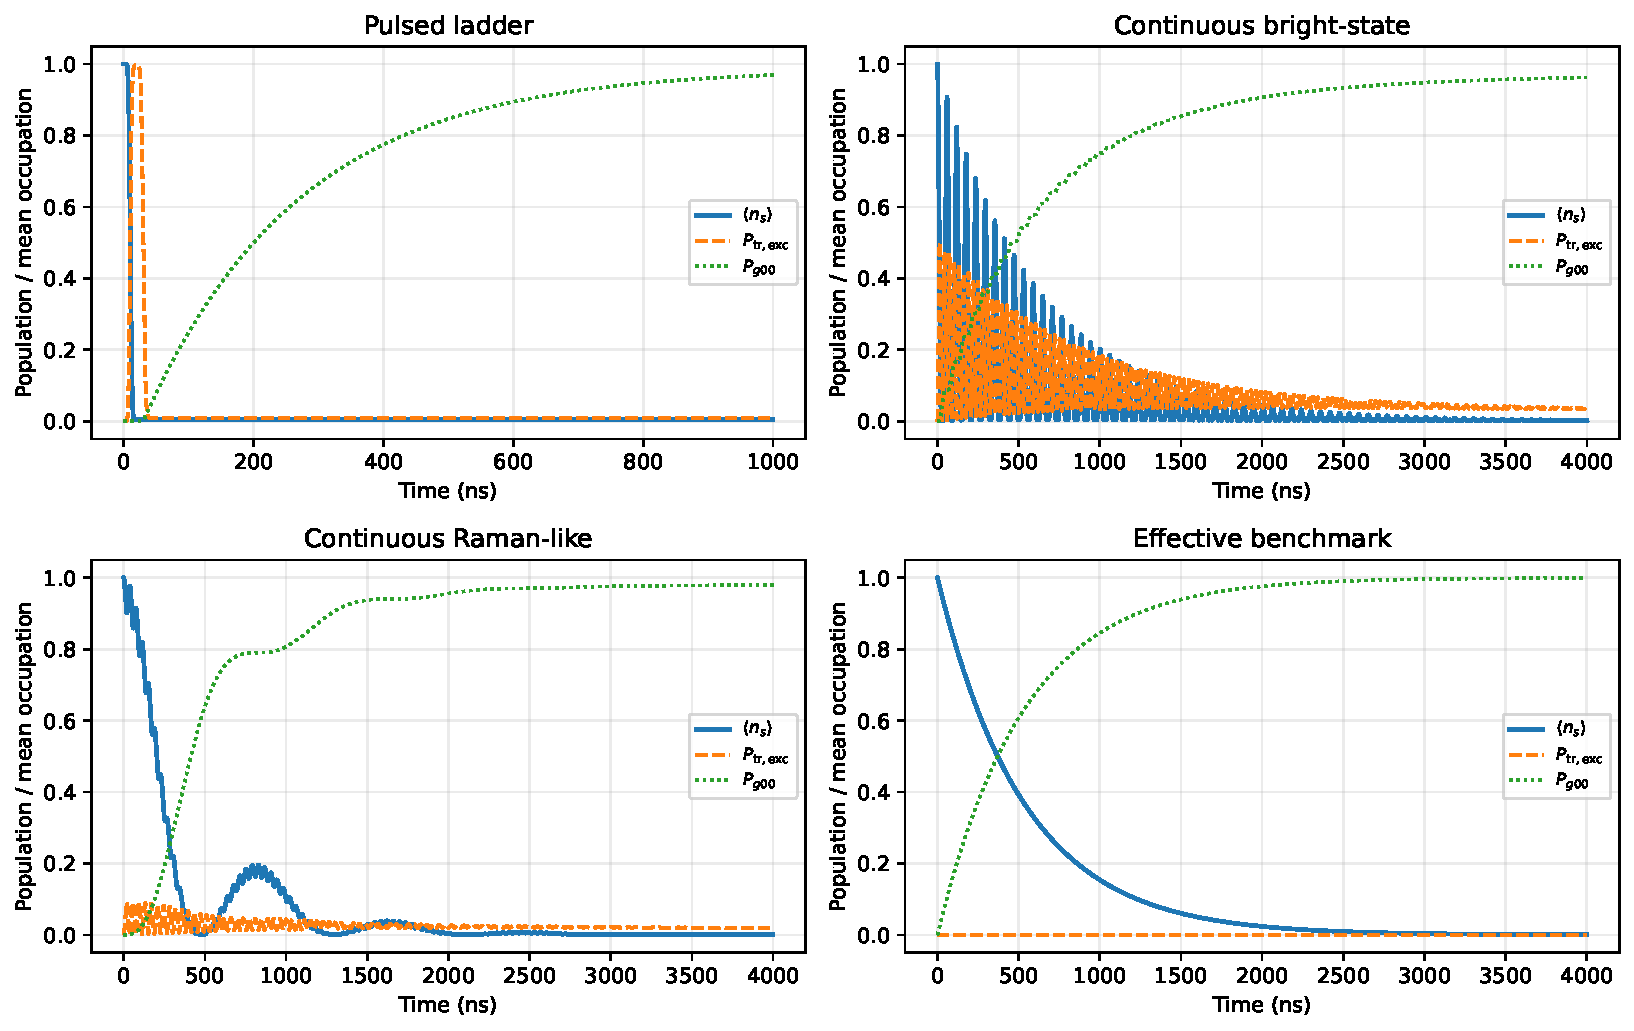
\includegraphics[width=\columnwidth]{../figures/scheme_cooling_dynamics.pdf}
\caption{Representative single-photon cooling trajectories for the four compared schemes. Each panel shows the storage occupation $\langle n_s\rangle$, transmon excited-state probability $P_{\mathrm{tr,exc}}$, and ground-vacuum probability $P_{g00}$ as a function of time. The pulsed ladder exhibits an $\SI{11}{ns}$ storage e-fold inside a full \SI{1000}{ns} pulse-plus-ringdown sequence, the bright-state protocol has $\tau_e \approx \SI{13}{ns}$, and the Raman-like protocol has $\tau_e \approx \SI{244}{ns}$. The effective benchmark ($\tau_e = \SI{535}{ns}$) is included as an idealized reference.}
\label{fig:dynamics}
\end{figure}

\begin{figure}[t]
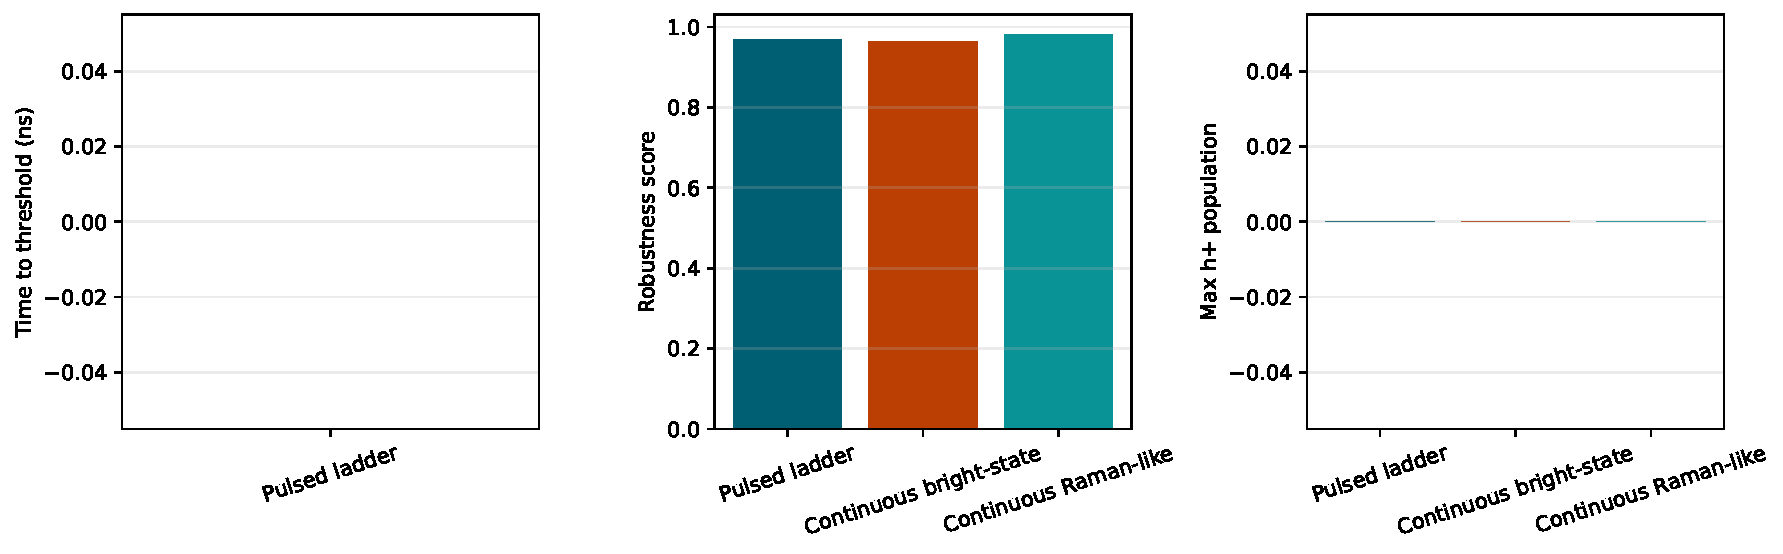
\includegraphics[width=\columnwidth]{../figures/scheme_comparison_summary.pdf}
\caption{Summary comparison of the three physical schemes. Left: e-fold cooling time $\tau_e$. Center: composite robustness score $R$ (Eq.~\ref{eq:robustness}). Right: final residual storage occupation $\langle n_s\rangle_{\mathrm{f}}$. The Raman-like protocol is slowest but achieves the highest robustness and lowest residual occupation.}
\label{fig:summary}
\end{figure}

\begin{figure}[t]
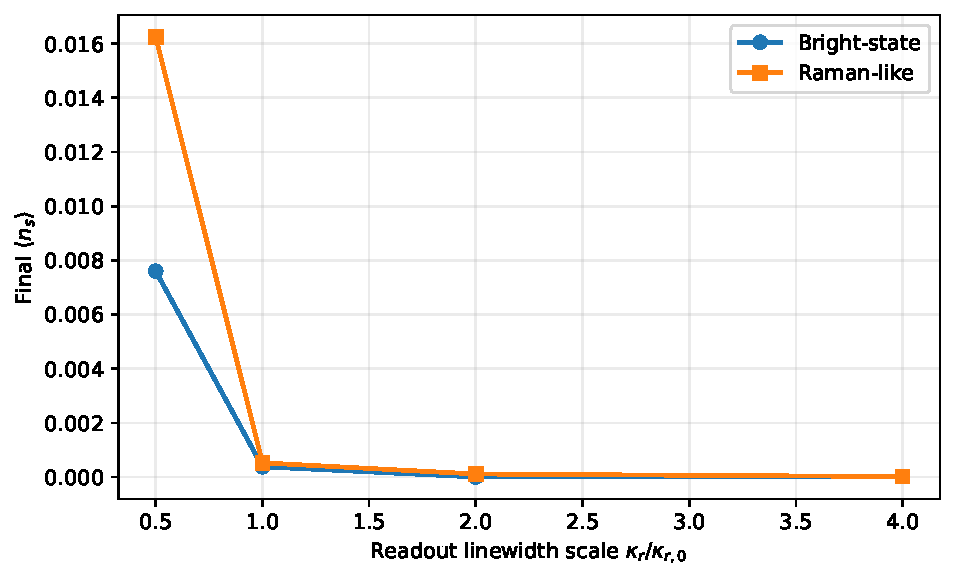
\includegraphics[width=\columnwidth]{../figures/readout_kappa_tradeoff.pdf}
\caption{Effect of readout linewidth on cooling performance for the two continuous schemes. Increasing $\kappa_r$ from $0.5\times$ to $4\times$ baseline reduces the Raman-like residual occupation by a factor of ${\sim}770$ and improves $P_{g00}$ from $0.960$ to $0.990$. The bright-state protocol also improves but with less dramatic gains.}
\label{fig:kappa}
\end{figure}

\begin{figure}[t]
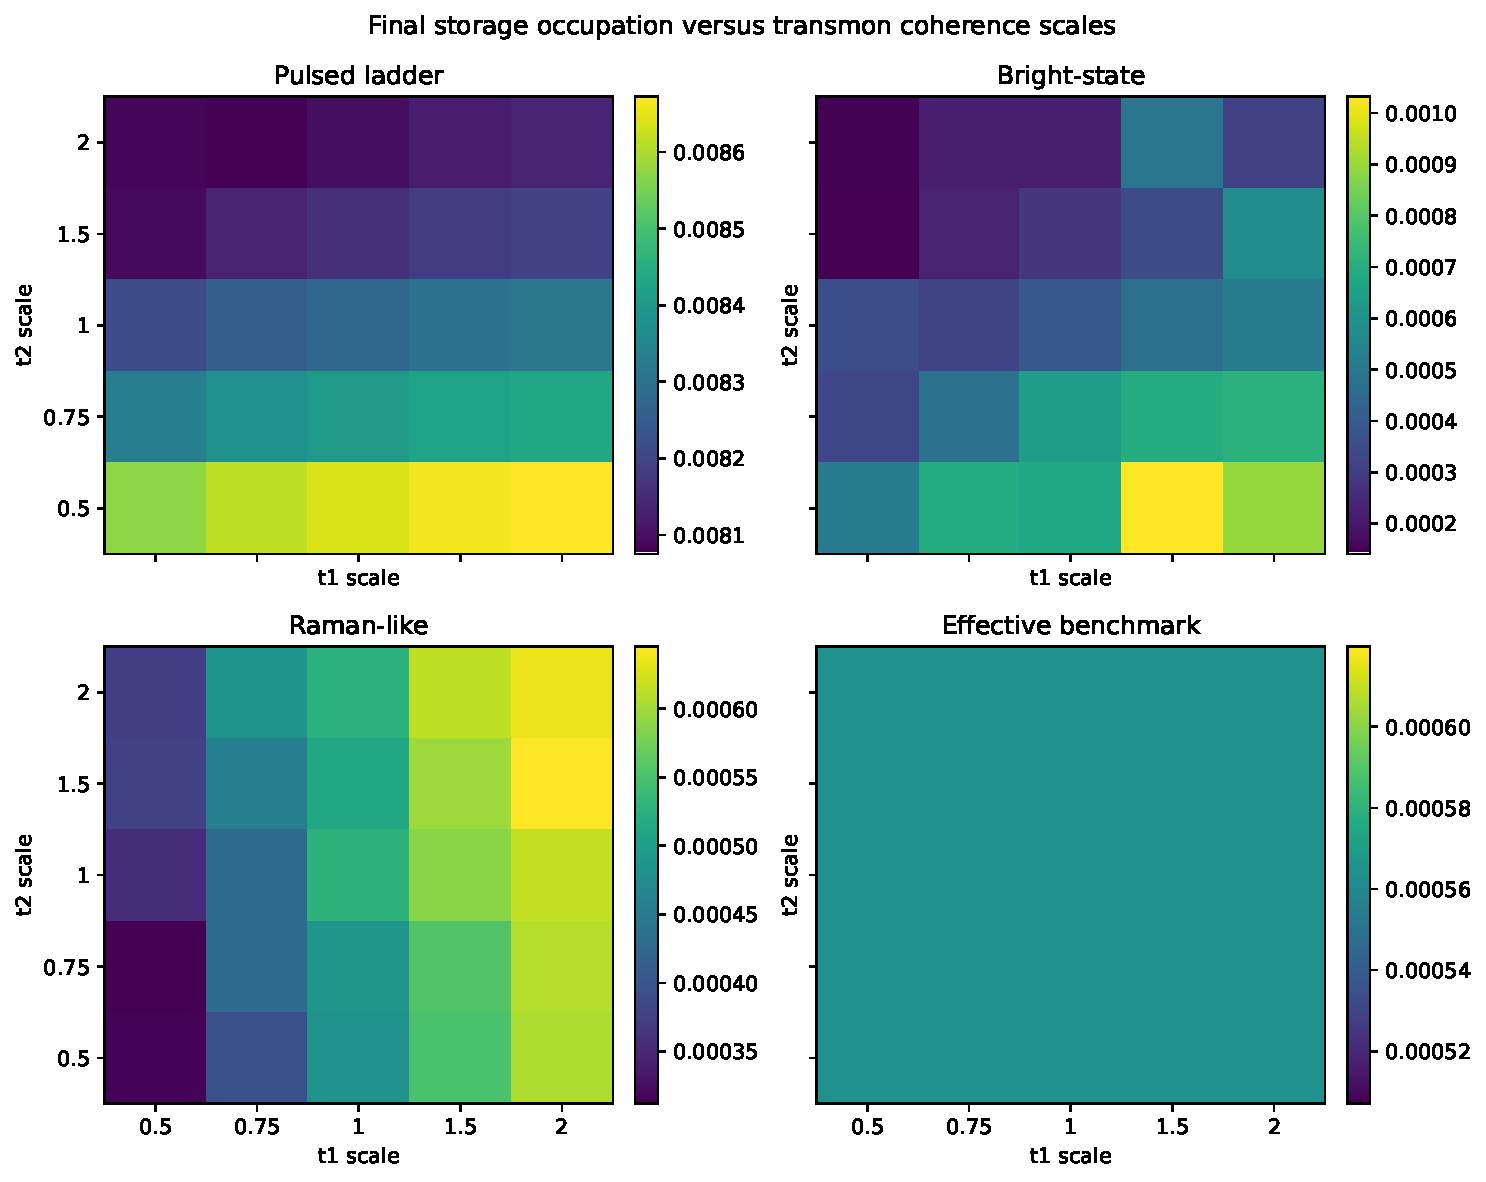
\includegraphics[width=\columnwidth]{../figures/coherence_robustness_heatmaps.pdf}
\caption{Coherence robustness heatmaps showing ground-vacuum probability $P_{g00}$ as a function of transmon $T_1$ and $T_2$ scaling factors for each physical scheme. The Raman-like protocol maintains $P_{g00} > 0.978$ across the full grid.}
\label{fig:coherence_heatmaps}
\end{figure}

\begin{figure}[t]
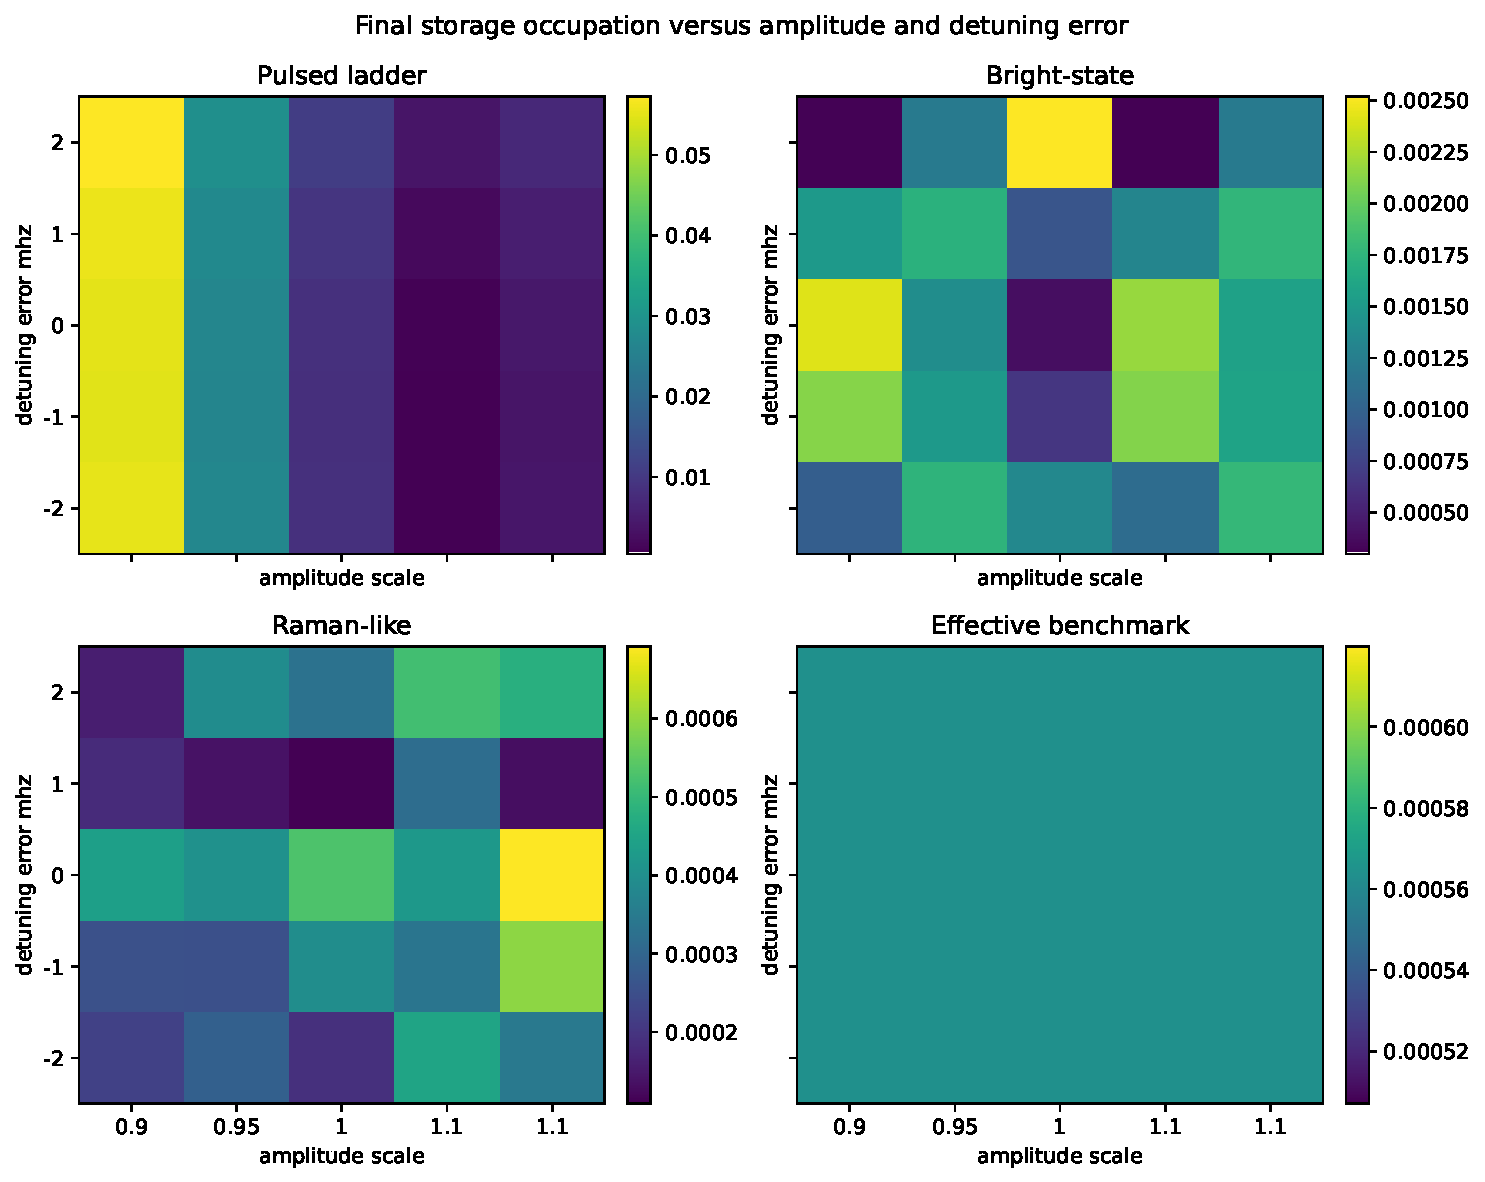
\includegraphics[width=\columnwidth]{../figures/calibration_robustness_heatmaps.pdf}
\caption{Calibration robustness heatmaps showing $P_{g00}$ as a function of amplitude scaling and detuning error. The pulsed ladder shows the widest $P_{g00}$ variation (minimum $0.868$), while the Raman-like protocol remains above $0.976$.}
\label{fig:calibration_heatmaps}
\end{figure}

\begin{figure}[t]
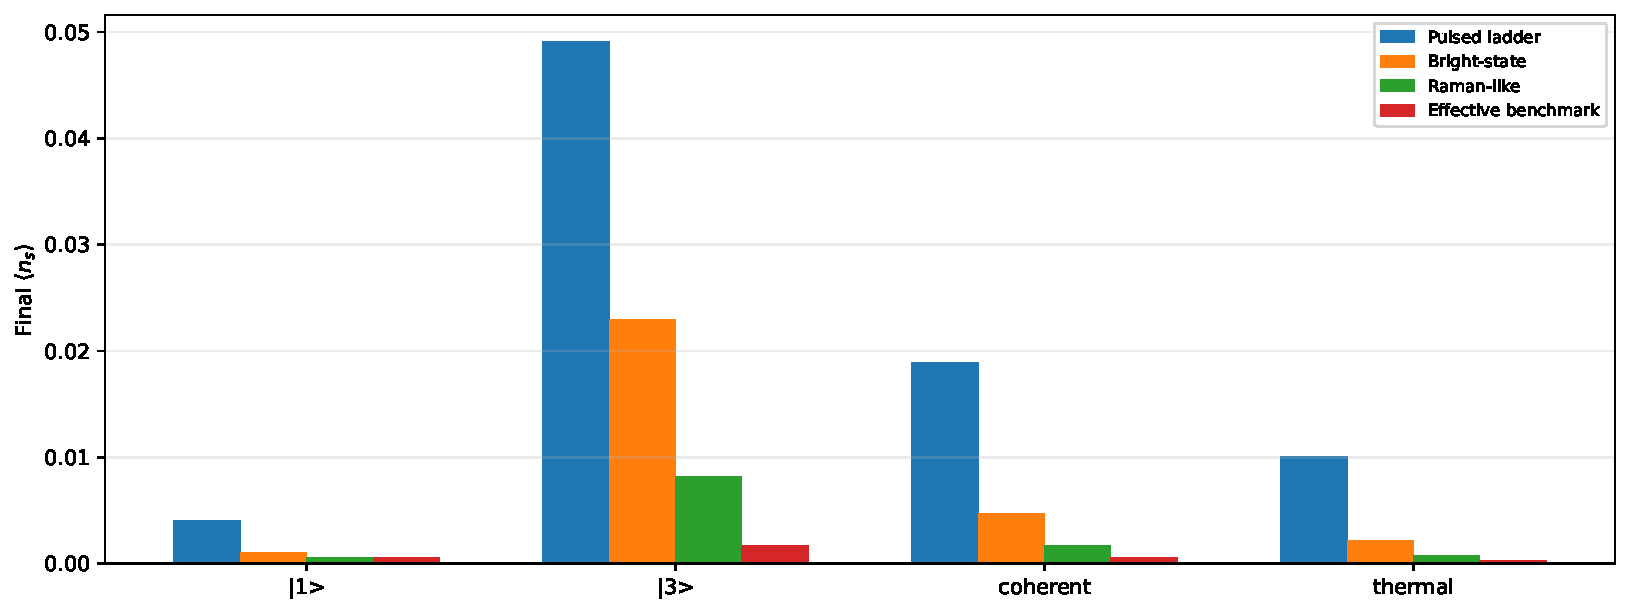
\includegraphics[width=\columnwidth]{../figures/initial_state_comparison.pdf}
\caption{Cooling performance across multiple initial states: $|1\rangle$, $|3\rangle$, coherent $|\alpha{=}1\rangle$, and thermal $\bar{n}=0.5$. The continuous schemes maintain consistent e-fold times across initial conditions, while the pulsed ladder scales linearly with Fock number.}
\label{fig:initial_states}
\end{figure}

\end{document}
